\documentclass[12pt]{article}
\usepackage{fullpage}
\usepackage{graphicx, rotating, booktabs} 
\usepackage{times} 
\usepackage{fbb} 
\usepackage{natbib} 
\usepackage{indentfirst} 
\usepackage{setspace}
\usepackage{grffile} 
\usepackage{hyperref}
\usepackage{tikz-cd}
 \usetikzlibrary{cd}
\usepackage[export]{adjustbox}
\usepackage[most]{tcolorbox}
\usepackage{verbatimbox}
\usepackage{lscape}
\usepackage{afterpage}
\usepackage{amsmath}
\usepackage[labelfont={bf},textfont=it,labelsep=period]{caption}
 \usepackage{multirow} 
\setcitestyle{aysep{}}
\usepackage{dcolumn}

\hypersetup{
  colorlinks = true,
  urlcolor = blue,
  linkcolor = black,
  citecolor = black,
  pdfauthor = {Joshua Alley},
  pdfkeywords = {},
  pdftitle = {},
  pdfsubject = {},
  pdfpagemode = UseNone,
%  pdffitwindow = true
%  pdfcenterwindow = true
}



\singlespace
\title{\textbf{Using Hierarchical Models to Estimate Heterogeneous Effects}}
\author{Joshua Alley \\
Assistant Professor \\
University College Dublin\thanks{Thanks to Carlisle Rainey for helpful comments.} \\
joshua.alley@ucd.ie
}

 
\date{\today}

\bibliographystyle{apsr}

\usepackage{sectsty}
\sectionfont{\Large}
\subsectionfont{\noindent\large\textit}
\subsubsectionfont{\normalsize}

\makeatletter
\renewcommand\tiny{\@setfontsize\tiny{9}{10}}
\makeatother


\begin{document}

\maketitle 

\begin{abstract} 
%Heterogeneous effects are common in social science. 
This note describes a Bayesian hierarchical approach to estimating heterogeneous effects. 
To begin, researchers specify groups and sources of heterogeneity based on quantities of interest such as heterogeneous treatments, treatment heterogeneity, and policy relevance.  
Then, researchers should fit a hierarchical model with varying slopes and intercepts by groups and group level factors modifying the slopes.
This captures systematic and random variation in heterogeneous effects, estimates effects within each group, and measures effect variance. 
Hierarchical modeling provides an intermediate tool between interactions or subgroup analyses and machine-learning approaches to discovering complex heterogeneity. 
It is more flexible than interactions and reduces the risk of underpowered subgroup comparisons.
At the same time, it is more theoretically driven and interpretable than some machine-learning approaches, as well as easier to implement in small datasets. 
Researchers should use hierarchical models alongside other approaches to understand heterogeneous effects for scholarship and policy.
\end{abstract} 


\newpage 
\doublespace 


\section{Introduction}


% one: het effects matter
Whether in observational and experimental studies, every independent variable social scientists examine impacts some units differently than others. 
Common estimands aggregate heterogeneous effects, sometimes in misleading ways.\footnote{For example, \citet{Abramsonetal2022} note that the average marginal component effect (AMCE) of conjoint experiments gives more weight to intense preferences.} 
Average effects can be useful, but they often obscure interesting and important variation. 


As a result, understanding heterogeneous effects is essential for policy and scholarship. 
Estimating heterogeneity allows scholars to clarify the connection between their independent variable and outcome.
Policymakers can maximize the impact of finite resources with targeted interventions. 
% expand/sharpen this, if there is space. (There is not for PA) 

% two: introduce my solution 
This note describes a hierarchical Bayesian approach to estimating heterogeneous effects. 
Before fitting a model, researchers define groups based on the potential sources of heterogeneity such as other treatments, context, demographics, or policy concerns. 
The model then estimates heterogeneous effects across those groups using varying slopes and intercepts, along with covariates that predict slopes.\footnote{These ideas are established in the statistics literature \citep{FellerGelman2015}, but political science researchers rarely use them. \citet{FellerGelman2015} have three applied political science citations, and of these only \citet{Marquardt2022} models treatment effects.} 
Modeling heterogeneous effects in this way produces easily interpretable results, which facilitates argument testing.
It also allows researchers to examine effects within groups, compare different sources of heterogeneous effects and describe how much an effect varies.  


Such hierarchical models are easy to fit using the brms package for \textsf{R}. 
I provide example code in this note and the appendix.
After fitting a model, researchers can calculate substantive effects with the marginaleffects package \citep{ArelBundockme}.


% three: loads of techniques
Hierarchical modeling of heterogeneous effects fills a niche between existing tools.
Parametric interactions and subgroup analyses are ubiquitous because they are easy to implement and interpret.
These approaches lose interpretability with more than three dimensions and are often underpowered \citep{Simmonsetal2011}.\footnote{\citet{BlackwellOlson2022} describe a lasso approach to interactions that falls between machine-learning and linear regressions.}
More recent work employs random forests \citep{GreenKern2012, WagerAthey2018}, support vector machines \citep{ImaiRatkovic2013}, and ensemble methods \citep{Grimmeretal2017, Kuenzeletal2019, Dorieetal2022}.
These machine learning algorithms capture complex patterns, but can be difficult to interpret and implement, especially in smaller datasets that are common in social science. 

 
Using a hierarchical model is more flexible than parametric interactions but more straightforward than machine learning approaches.  
It preserves a simple and interpretable structure, while accommodating more factors and reducing the risks of subgroup analysis. 
Unlike some machine-learning techniques, this facilitates argument testing.
The hierarchical approach lacks the flexibility to discover high-dimensional heterogeneity, however.  
As a result, hierarchical modeling complements other heterogeneous effects techniques, and could contribute to ensemble models. 


% wrap and introduce the application 
In the remainder of this note, I describe the approach and demonstrate how it works by analyzing a study of how military alliances shape public support for war by \citet{TomzWeeks2021}. 
The reanalysis also reveals that alliances increase support for intervention most among men who support international engagement but are otherwise skeptical of using force. 
This suggests that alliances increase mass support for war by impacting individuals who otherwise prefer peaceful collaboration. 



\section{A Hierarchical Model of Heterogeneous Effects}


There are two steps in this approach to heterogeneous effects estimation. 
First, researchers must define the groups over which an independent variables' impact varies. 
To do this, they create groups based on unique combinations of characteristics such as other treatments, context and demographics.


Setting groups is the most important task.
This determines what heterogeneous effects a model estimates. 
Defining groups before model fitting helps researchers define what variation is most important, link heterogeneous effects to theory, and structure their analyses.\footnote{It also facilitates pre-registration when applicable.}
Poorly defined groups will obfuscate the results and can hinder model fitting.   


Researchers should create groups based on what variation is most important and interesting. 
Theory, policy concerns, or normative factors are all possible motivations.
Three general approaches follow from these factors.  


% three ways to set groups
First, researchers can set groups using combinations of other treatments, especially when an intervention has several dimensions but theory emphasizes one of them. 
The experimental design determines groups in this approach, and the results estimate heterogeneous treatments.   
For instance, if researchers want to know how different issues shape the impact of elite cues \citep{GuisingerSaunders2017}, they could define groups by issues. 


A second approach uses unit and contextual factors to create groups and estimate treatment effect heterogeneity. 
In this instance, researchers examine what within or around units shapes a treatment.
For example, \citet{Alley2021isq} uses alliance characteristics to examine when alliance membership increases or decreases military spending.


Third, researchers can emphasize policy aims.
Understanding how an intervention impacts a specific population is a common problem.
Researchers might want to know if a job-training program improves employment prospects for black women in the South, for instance.  


% grouping factors: numbers 
Whether researchers use other treatments, context, or policy to determine groups, the number of grouping factors depends first on theory.
There are some practical constraints, however.
Dividing groups based on many factors will create many small groups and increase the risk of model fitting problems. 
Using only one factor will create an unidentified model, and researchers should use interactions in that case. 


After defining groups, researchers fit a hierarchical model of effects within the groups.\footnote{Bayesian estimation is easiest. Priors depend on the problem and researcher knowledge.} 
The first equation links the treatment and outcome. 
The second equation estimates heterogeneous effects as a function of the group characteristics.\footnote{Researchers can adjust for autocorrelation and clustering as needed.}  


This model can apply to many problems, but for ease of exposition consider making between-unit comparisons based on an experimental treatment.    
Start with \textit{N} units indexed by \textit{i}, some of which receive a binary treatment \textit{T}.
For simplicity, assume that the outcome variable ${y}$ is normally distributed with mean $\mu_i$ and standard deviation $\sigma$.\footnote{Researchers should use binary, categorical and other outcome likelihoods as needed.}
\textit{g} indexes researcher-defined groups. 


The first equation predicts the outcome mean. 
The outcome for each unit is then a function of varying intercepts $\alpha_g$, an optional matrix of control variables \textbf{X},\footnote{Adding additional grouping structures for more complex data is also straightforward.} and a set of group treatment effects $\theta_g$, which are normally distributed with mean $\eta_g$ and standard deviation $\sigma_\theta$. 
The researcher divides all units into \textit{g} groups based on unique combinations predictors of heterogeneous effects \textbf{Z}. 
Each $\theta$ parameter estimates the treatment effect in group \textit{g}, and is often referred to as a varying slope. 


\begin{equation}
\begin{aligned}
y_i &\sim N(\mu_i, \sigma) &\text{(Likelihood)} \\
\mu_i &= \alpha + \alpha_g + \theta_g \textit{T} + \textbf{X} \beta &\text{(Outcome Equation)}  \\
\theta_g &\sim N(\eta_g, \sigma_\theta) \\ 
\eta_g &= \lambda_0 + \textbf{Z} \lambda &\text{(Heterogeneous Effects)} 
\end{aligned}
\end{equation}


The second equation then predicts the treatment effects with the matrix \textbf{Z}, which contains unique combinations of whatever variables define the groups.  
As a result, each $\theta$ reflects a unique mix of factors that modify the treatment.
The second equation also includes an intercept $\lambda_0$ that estimates the impact of treatment when all sources of heterogeneity are zero.\footnote{In brms for a model with no controls and two variables modifying the impact of a treatment, the model formula is simply y $\sim$ 1 + treat*(var1 + var2) + (1 + treat | var1:var2). treat*(var1 + var2) expresses part of the second equation, while (1 + treat | var1:var2) lets slopes vary by group.}


% Interpretation 
Modeling heterogeneous effects across groups facilitates detailed inferences about how much and why an effect varies.
First, the $\theta$ parameters estimate the impact of a variable within each group.\footnote{The random intercepts $\alpha_g$ and varying slopes $\theta_g$ should usually have a common multivariate normal prior to capture correlations between group slopes and intercepts.}
All $\theta$s reflect a systematic component from \textbf{Z} $\lambda$ and a random component of varying slopes from $sigma_\theta$. 
The systematic component will usually dominate. 


% additional information 
In addition to group-specific effect estimates, a hierarchical model estimates how specific factors drive differences between groups via the $\lambda$ parameters.
This facilitates rich description of effects across groups. 
The $\sigma_\theta$ parameter also summarizes how much the effects vary. 
Other techniques such as OLS with robust standard errors provide far less information.


% advantages 
Estimating heterogeneous effects in this way has three advantages.
First, this model allows researchers to make detailed inferences about heterogeneous effects in an easy to interpret framework. 
Researchers can thus examine theories of heterogeneous effects and compare sources of variation.\footnote{Rescaling variables in the heterogeneous effects equation can aid model fitting and coefficient comparisons \citep{Gelman2008}.} 
Partial pooling also facilitates reasonable estimates for small groups by sharing information across groups and leveraging the predictors in the heterogeneous effects equation. 
Finally, this approach will be faster than machine learning approaches for many datasets, easier to use in small datasets, and may scale better than models that attempt to estimate individual treatment effects.


% disadvantages
Like all methods, the hierarchical approach has downsides, some of which can be ameliorated by altering the basic framework above. 
Because groups are based on unique combinations of heterogeneous effect variables, using multiple continuous variables in the heterogeneous effects equation creates many small groups or individual treatment effects, which increases the risk of sampling problems, especially in small datasets. 
If using several continuous variables hinders model convergence, researchers can bin continuous variables.


Furthermore, unlike machine learning approaches, this model will not uncover high-dimensional interactions. 
Even so, researchers can inject substantial flexibility by using additional interactions or non-linear specifications in either level of the model. 
Finally, this model can show general trends, but will not make powerful comparisons between every groups. 
Researchers who want to compare specific groups may lack empirical leverage, especially if the groups are small.



\section{Example Application} 


In the following, I demonstrate how the hierarchical approach works by reanalyzing a study by \citet{TomzWeeks2021} (TW hereafter). 
TW examine how military alliances shape public support for war.
In a factorial experiment with vignettes, they find that alliances increase support for war by 33\% on average. 
This is a large and potentially important effect. 
I use a hierarchical model to estimate how demographics drive treatment heterogeneity.\footnote{See the appendix for a heterogeneous treatments analysis that corroborates TW's results.}


Here, race, gender, hawkishness and internationalism define the groups and predict the impact of alliances on support for using force. 
I selected these variables because foreign policy dispositions like militant assertiveness shape general willingness to intervene \citep{Kertzeretal2014} as do gender \citep{Barnhartetal2020} and race. 
I also control for other experimental manipulations. 


I describe the results in two ways. 
First, I summarize the correlates of alliance impact in \autoref{fig:tw-het-source}.
I then present the corresponding heterogeneous effects for each group in \autoref{fig:tw-treat-het}.


\begin{figure}[htpb]
	\centering
		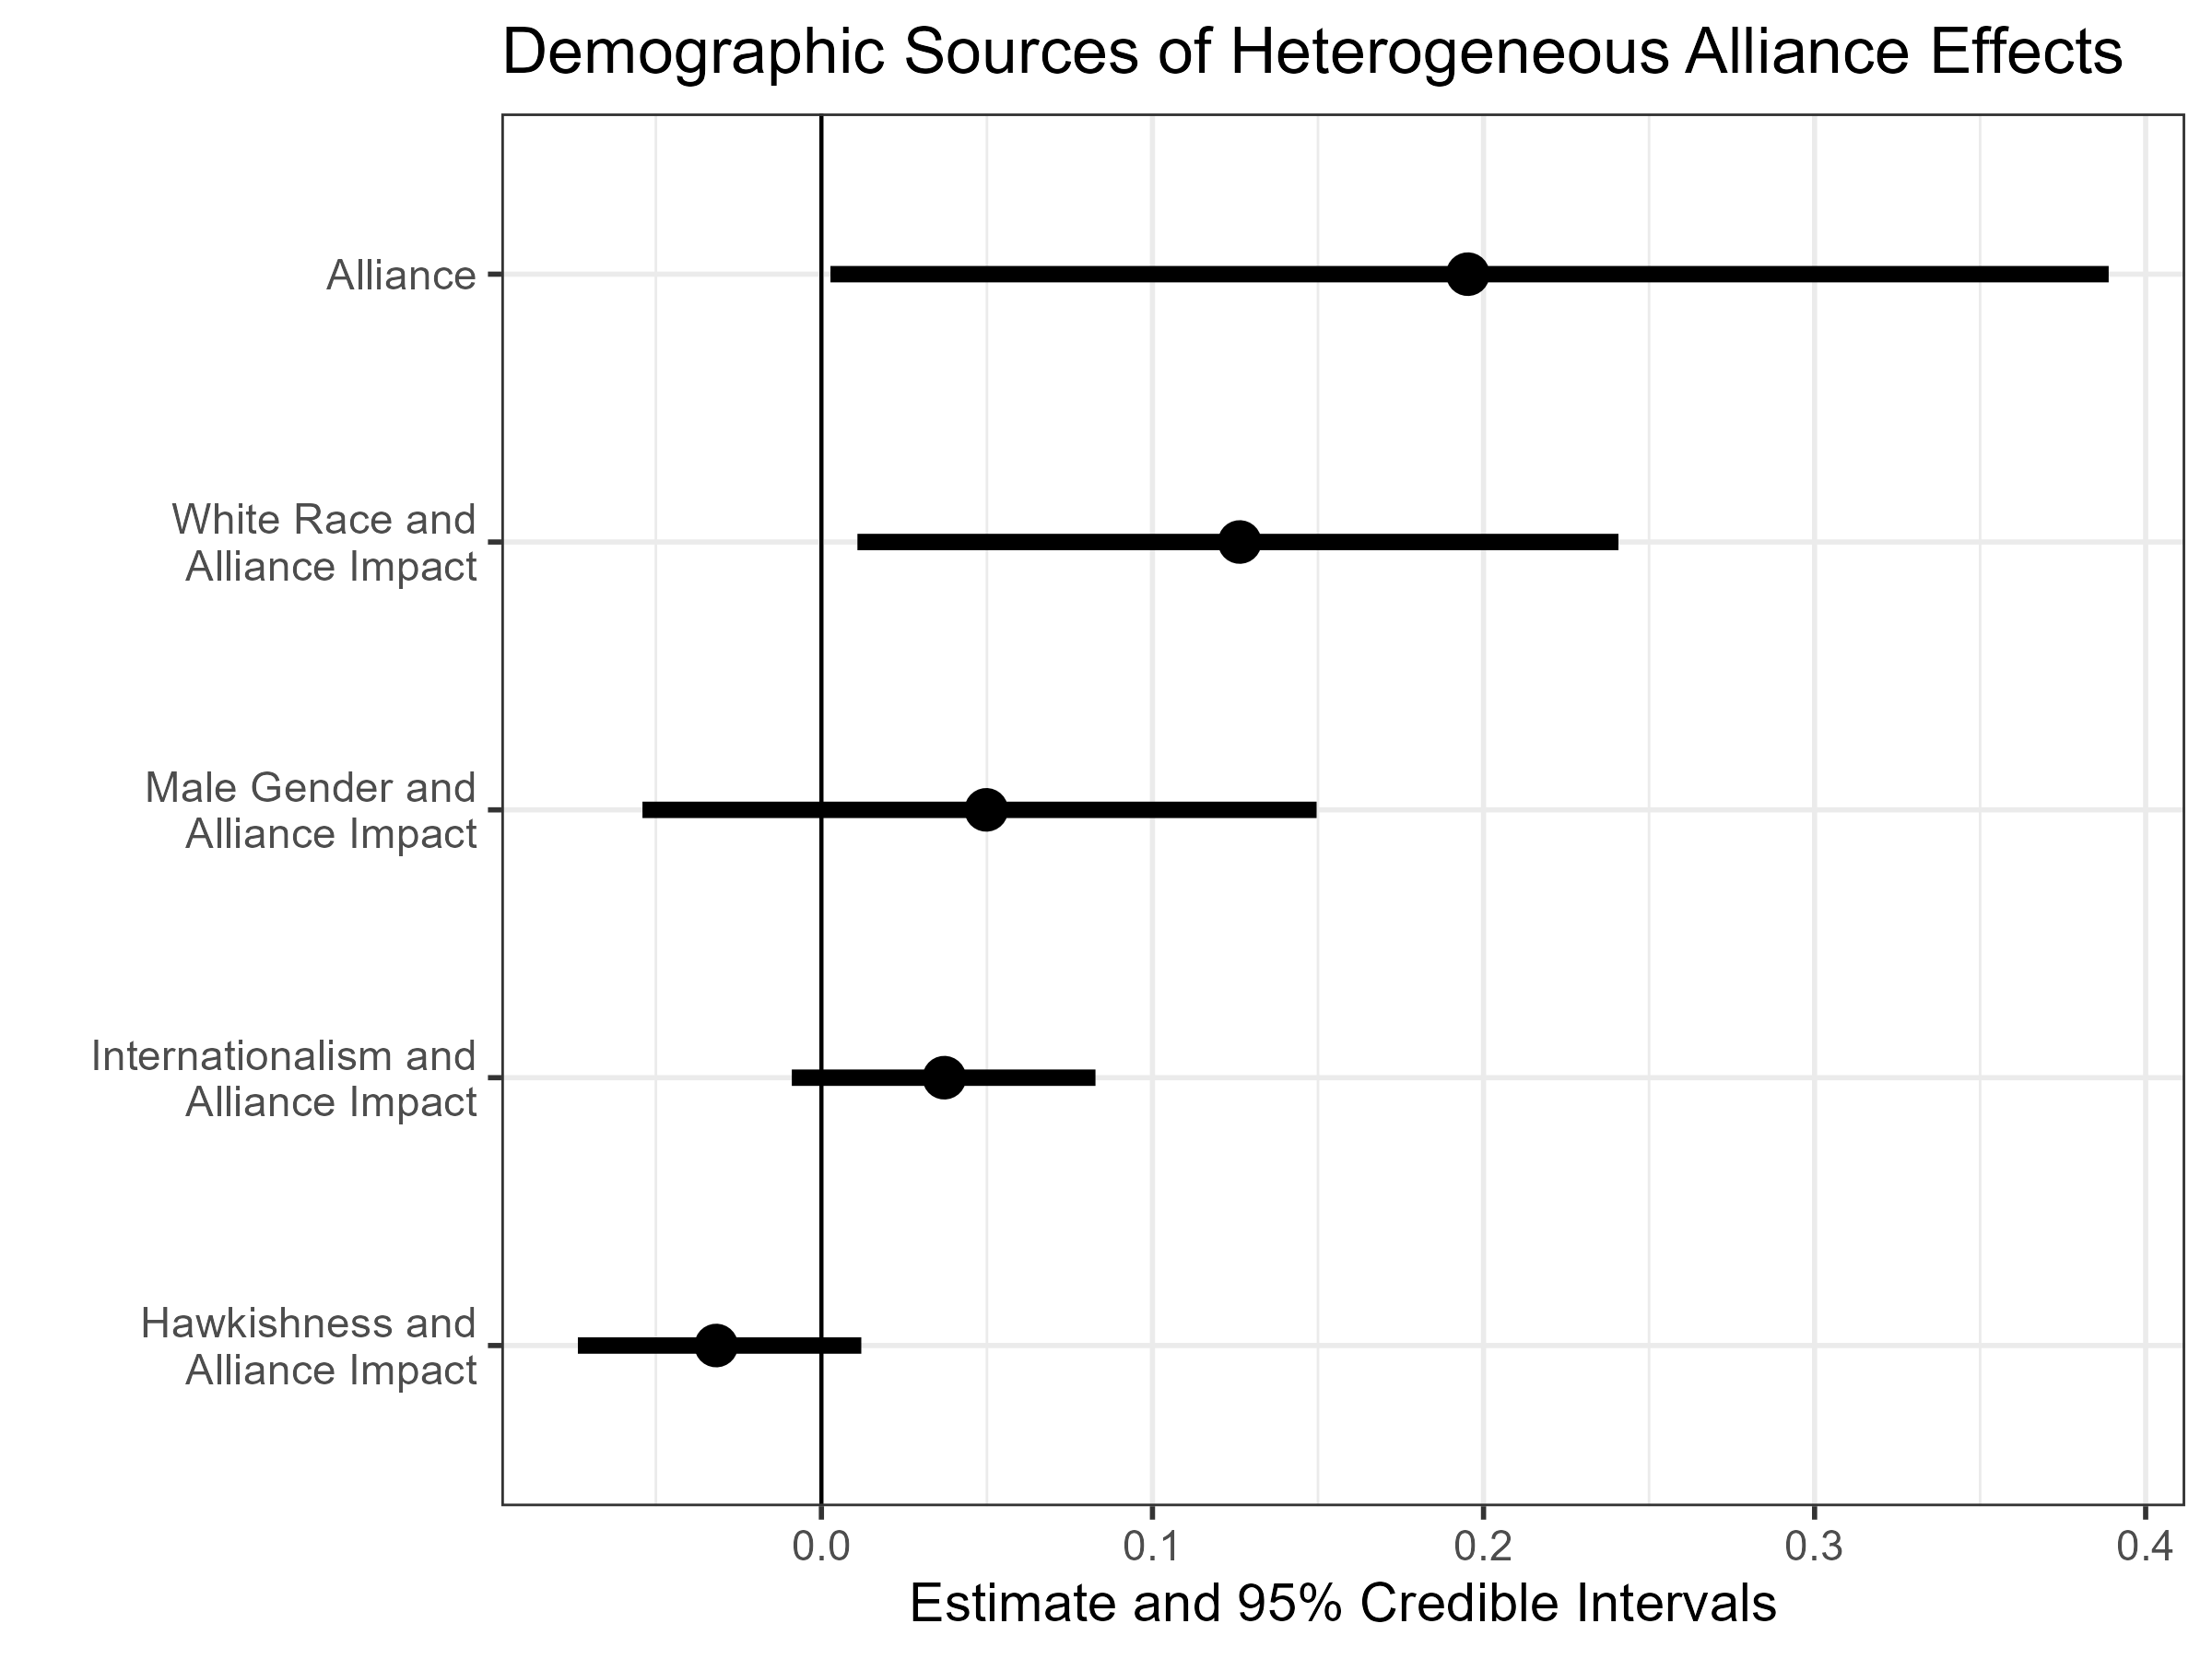
\includegraphics[width=0.95\textwidth]{../figures/tw-het-source.png}
	\caption{Heterogeneous effects equation coefficients from a hierarchical model of how military alliances impact public support for war. Hawkishness, internationalism, white race and male gender predict the impact of alliances.}
	\label{fig:tw-het-source}
\end{figure}


\autoref{fig:tw-het-source} shows how internationalism, hawkishness, race and gender modify the impact of alliances.\footnote{These are the $\lambda$ parameters above.}
When all other variables are 0, alliances increase support for intervention by 20\%. 
That impact is 12\% greater among white respondents. 
As internationalism increases, the impact of alliances rises by 4\% in expectation.
Greater hawkishness marginally attenuates the impact of an alliance. 
Furthermore, there is an additional 5\% of variation in the alliance impact that these systematic components do not explain.\footnote{This is $\sigma_\theta$ above.}


\begin{figure}[htpb]
	\centering
		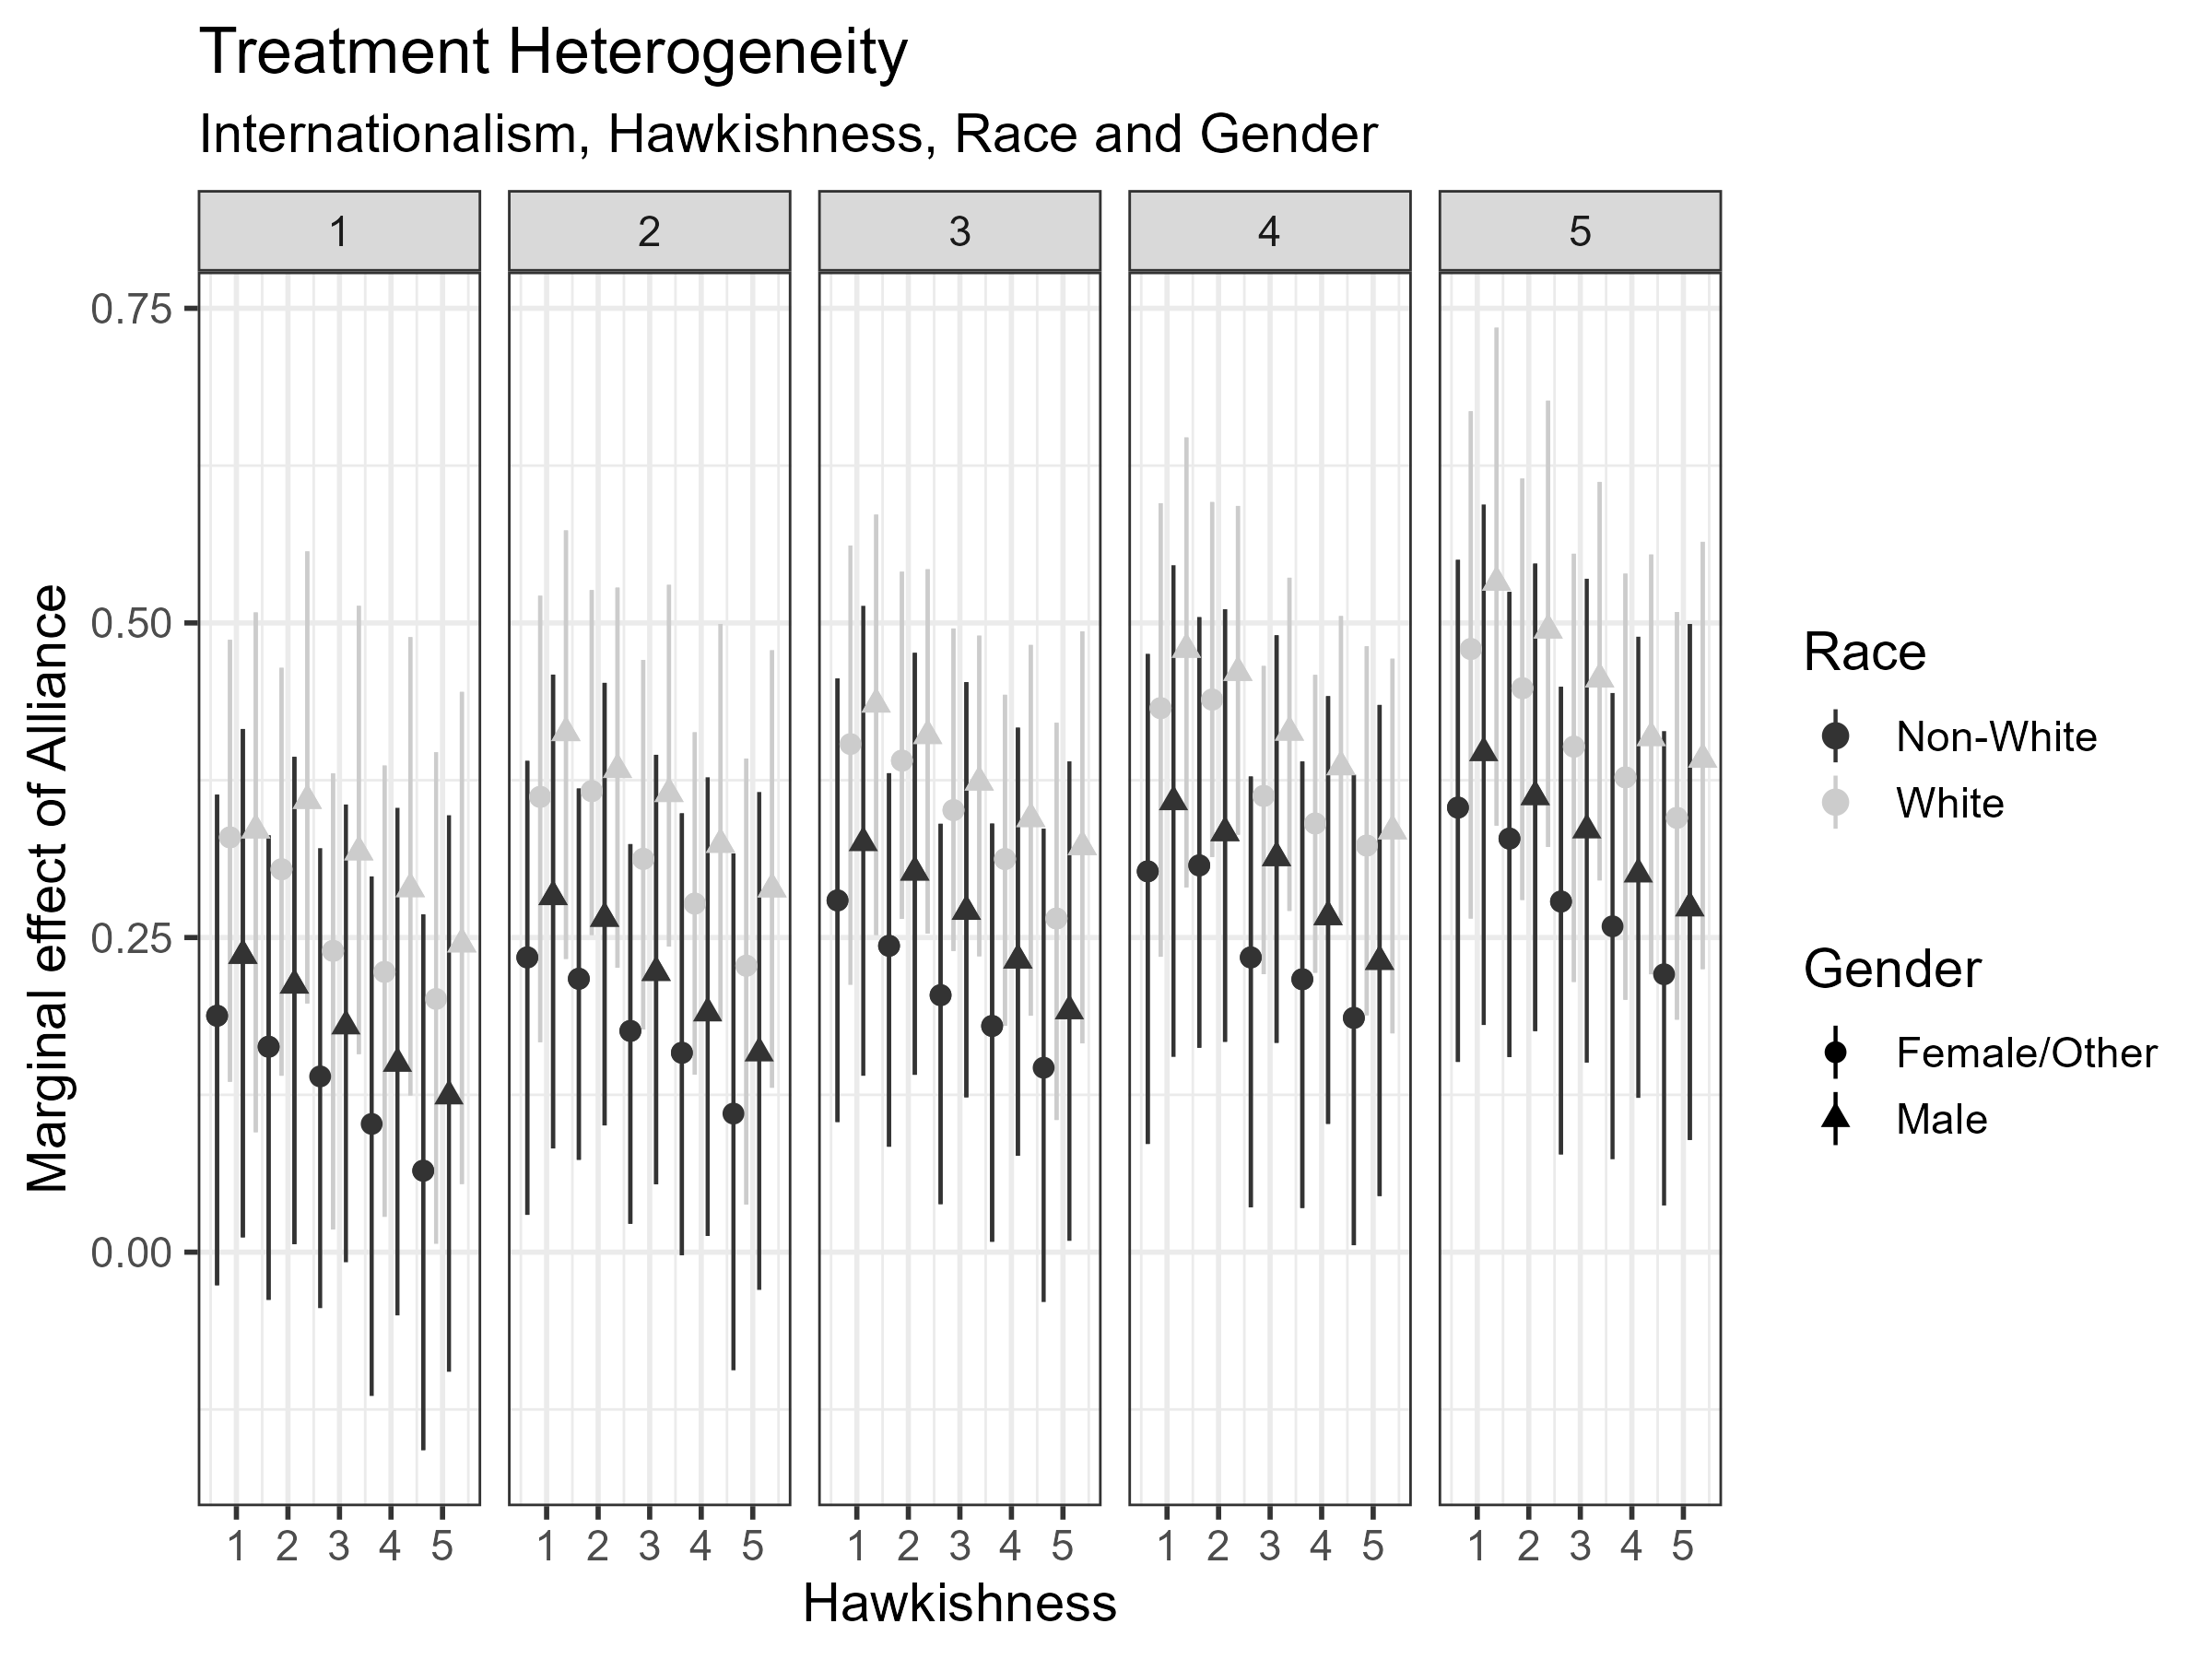
\includegraphics[width=0.95\textwidth]{../figures/tw-treat-het.png}
	\caption{Estimates of how the impact of military alliances on support for using force varies across different demographic groups. Points mark the posterior median and bars summarize the 95\% credible interval.}
	\label{fig:tw-treat-het}
\end{figure}


\autoref{fig:tw-treat-het} shows that alliances exert the most influence on support for foreign interventions among white men, especially those with low hawkishness and high internationalism, who can be labeled as ``cooperative internationalists.'' 
Among white men with minimum hawkishness and maximum internationalism, alliances increase support for using force by 50\%, which is roughly double the typical effect. 
By contrast, alliances have little impact on support for war among non-white females who are skeptical of international engagement.
Militant assertiveness reduces the impact of alliances, perhaps because these individuals support intervention regardless. 
This implies that alliances help convince individuals who back international engagement but are less inclined to use force. 
As a result, internationalism is more important than hawkishness for understanding who is willing to fight for U.S. allies. 


% variation
How much does the impact of alliances vary?
The minimum impact of alliances is .06, and the maximum is .53, and median is .3. 
The standard deviation of the impact of alliances is .09. 
Alliances never decrease support for intervention, but how much they increase support varies widely across demographic groups. 



These results show some of the strengths and weaknesses of the hierarchical approach to estimating heterogeneous effects.\footnote{In the appendix, I analyze \citet{BushPrather2020}.}
A simple model based on demographic groups provides new insights about who responds to alliances. 
At the same time, because some demographic groups are small, the within-group effect estimates have substantial uncertainty, so comparing groups is challenging. 
Smaller groups would have less uncertainty but perhaps obscure variation in the impact of alliances. 


\section{Conclusion}

This note introduced a simple and interpretable hierarchical technique for estimating heterogeneous effects. 
The approach above can apply to a wide range of outcomes, data structures, and theories. 
Explicitly modeling how different groups respond to an independent variable can help test arguments and inform policy.  


Hierarchical modeling provides an intermediate approach between simple interactions or subgroup analyses and complex machine-learning algorithms. 
As a result, this technique complements existing tools and should not replace them. 
Researchers can use hierarchical models to check and inform other techniques, for instance by seeing if a key interaction holds when there are multiple modifiers. 
With this and other tools, scholars and policymakers can better understand heterogeneous effects.


\singlespace
 
\bibliography{../../MasterBibliography} 


%\documentclass[12pt]{article}

\usepackage{fullpage}
\usepackage{graphicx, rotating, booktabs} 
\usepackage{times}
\usepackage{fbb} 
\usepackage{natbib} 
\usepackage{indentfirst} 
\usepackage{setspace}
\usepackage{grffile} 
\usepackage{hyperref}
\usepackage{adjustbox}
\usepackage{multirow} 
\usepackage{amsmath}
\usepackage[labelfont={bf},textfont=it,labelsep=period]{caption}
\setcitestyle{aysep{}}
\usepackage{sectsty}
% for the big table
\usepackage{afterpage}
\usepackage{array}
\usepackage{lscape}
\usepackage{longtable}
\usepackage{float}
\sectionfont{\Large}
\subsectionfont{\noindent\large\textit}
\subsubsectionfont{\normalsize}


\singlespace
\title{\textbf{Appendix: Using Hierarchical Models to Estimate Heterogeneous Effects}}

\date{}
\bibliographystyle{apsr}

\begin{document}


\maketitle 

\singlespace 

\tableofcontents



\section{Tomz and Weeks Reanalysis}

This summarizes a heterogeneous treatments model of \citep{TomzWeeks2021} and details the underlying \textsf{R} code. 

\subsection{Heterogeneous Treatments} 

Here, I examine how the impact of alliances varies with other factors in the experiment, especially costs, stakes, region and partner democracy.
The heterogeneous treatment model corroborates TW's conclusion that alliances exert the greatest impact in instances when public opinion is otherwise skeptical of intervention.

\autoref{fig:tw-het-treat} supports TW's findings that alliances exert the most influence in situations where the public is otherwise unlikely to intervene. 
This figure shows the impact of alliances in unique combinations of all other experimental treatments. 
For a hypothetical democracy in Eastern Europe where intervention has high stakes, alliances exert minimal impact on public attitudes. 
In low-stakes and high cost interventions to support African, Asian or Latin American dictators, alliances increase support for intervention by 50\%. 
Beyond these systematic differences, random variation that is not attributed to the other treatments is roughly 6\%. 


\begin{figure}[htpb]
	\centering
		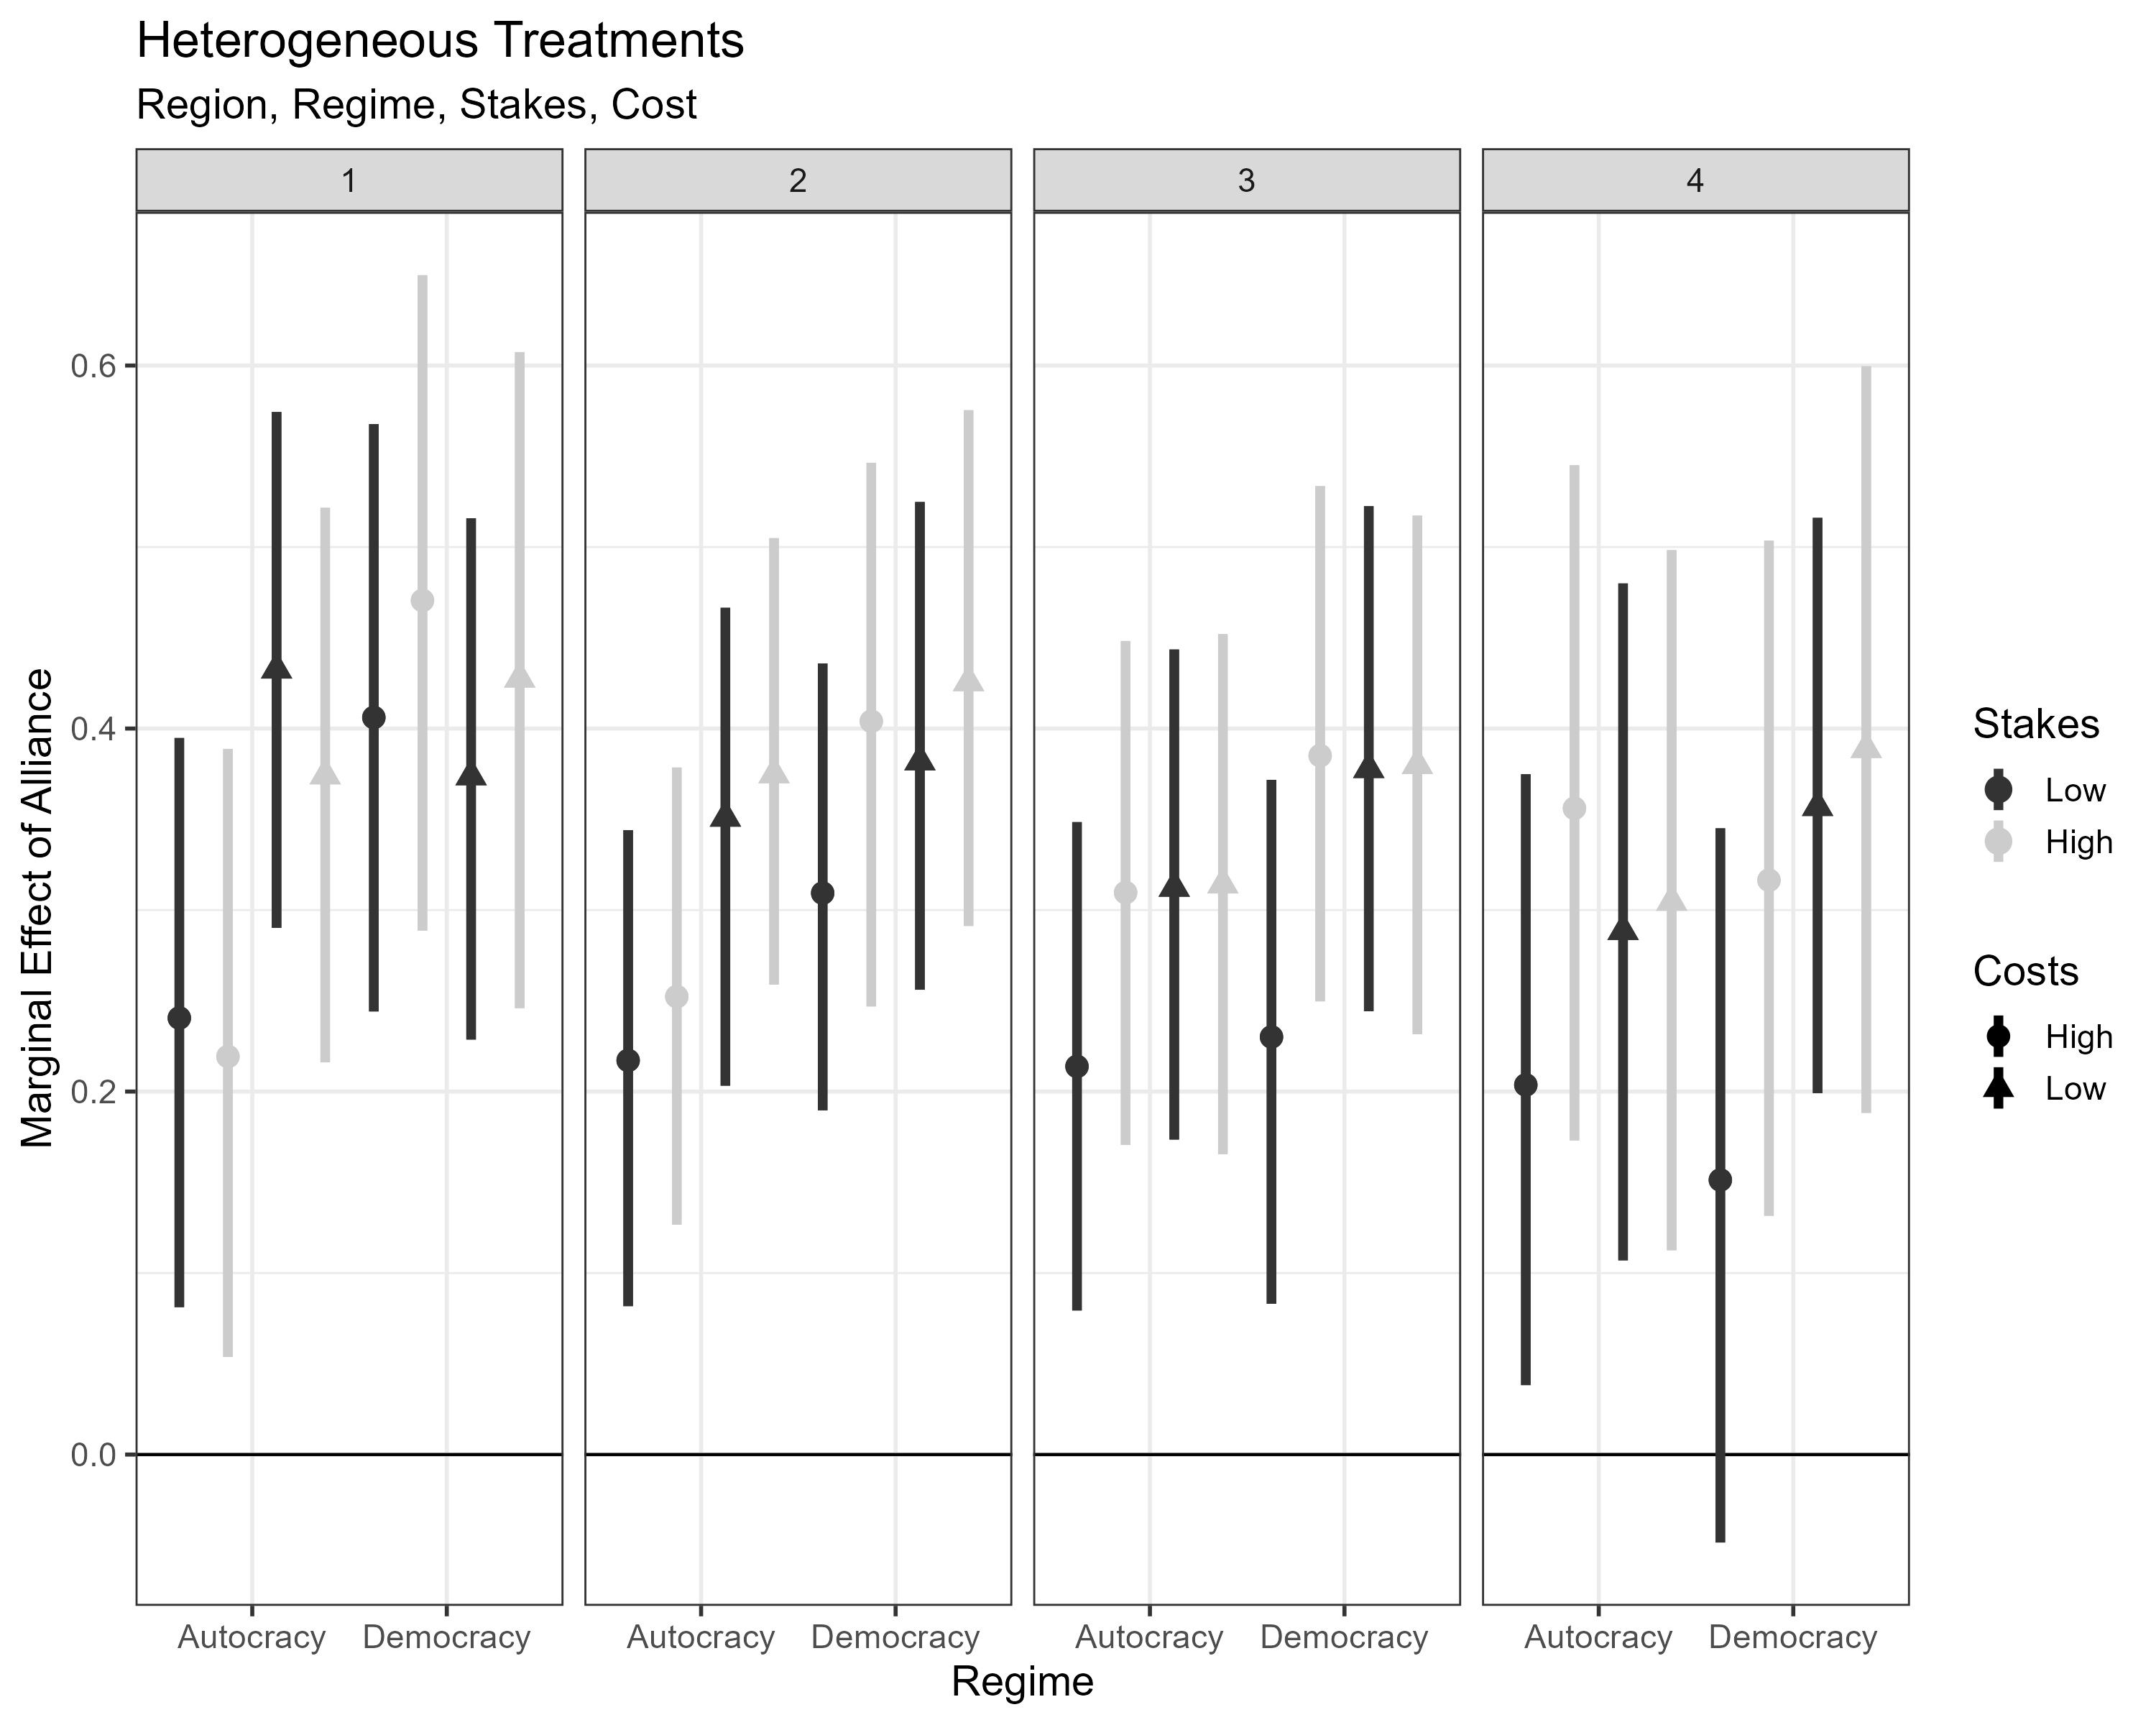
\includegraphics[width=0.95\textwidth]{tw-het-treat.png}
	\caption{Estimated impact of military alliances on public support for war across hypothetical region, costs, stakes and partner regime. Colors distinguish stakes, point shapes mark different costs, and estimates are grouped by regime type. Point estimates give the posterior median and error bars summarize the 95\% credible interval.}
	\label{fig:tw-het-treat}
\end{figure}


\subsection{R Code: Tomz and Weeks Reanalysis}

First, the following model formula expresses a heterogeneous treatments model where the impact of alliances varies with the regime under attack, the stakes, the costs, and the region. 
The \verb+treat.group+ indicator marks unique combinations of the regime, stakes, costs and region variables. 
It can also be written as \verb+regime:stakes:costs:region.txt+. 
I also control for gender, race, and three foreign policy dispositions. 

\begin{verbatim}
bf(force ~ 1 + white + male + hawk + intl + natl.sup + 
             alliance*(regime + stakes + costs + region.txt) + 
             (1 + alliance | treat.group) 
\end{verbatim}


The second formula expresses a treatment heterogeneity model where the impact of alliances varies with gender, race, and three foreign policy dispositions. 
The \verb+het.group+ indicator marks unique combinations of the demographic modifiers.
It can also be written as \verb+white:male:intl:hawk+. 
In this model, the other experimental conditions are controls. 

\begin{verbatim}
bf(force ~ 1 + regime + stakes + costs + region.txt +
             alliance*(white + male + intl + hawk) +
             (1 + alliance | het.group) 
\end{verbatim}



\section{Bush and Prather Reanalysis}


In the following, I again demonstrate how the model works by reanalyzing a study by \citet{BushPrather2020} (BP hereafter). 
This study examines how foreign meddling in elections impacts support for economic engagement with the meddler. 
One of their experiments examines how Russian or German engagement in the 2016 US election impacts mass support for trade and investment with those countries.
I use a heterogeneous effects model to check their results and further explore their findings. 


% describe design
BP employ a 2x2x2 factorial experiment.
This design randomizes whether a foreign country is interfering in the 2016 election, the country and their attitude towards Trump and whether the potential economic ties entail greater trade or investment in the United States.
In one treatment, Russia expresses support for Trump and in the other, Germany expresses opposition to Trump. 


BP hypothesize that individuals will prefer economic engagement with states that support their candidate. 
They thus examine how the impact of side-taking varies with the direction of the endorsement, individual political preferences, and the economic issue. 
To do this, they use four tables and figures, and rely on eight t-tests of differences in means between groups of roughly 25 respondents. 


The heterogeneous effects model encapsulates the argument and all tests by estimating the impact of side-taking on economic engagement as a function of which country is involved, a dummy indicator of intention to vote for Clinton, and their interaction. 
The interaction captures the hypothesis that Clinton voters will support engagement with Germany because Germany opposed Trump, and should be positive. 
I also add an indicator of whether the experiment deals with trade or investment. 
The heterogeneous effects equation also includes indicators of female gender and political engagement. 
The political engagement measure is a sum of political knowledge and interest. 


The outcome variable is a scale from one to four that measures support for greater economic engagement with the potential partner. 
To approximate BP's analyses, I use a normal outcome likelihood. 
Because this experimental randomization produced a roughly balanced sample, I do not include any control variables in the outcome equation. 


\begin{figure}[htpb]
	\centering
		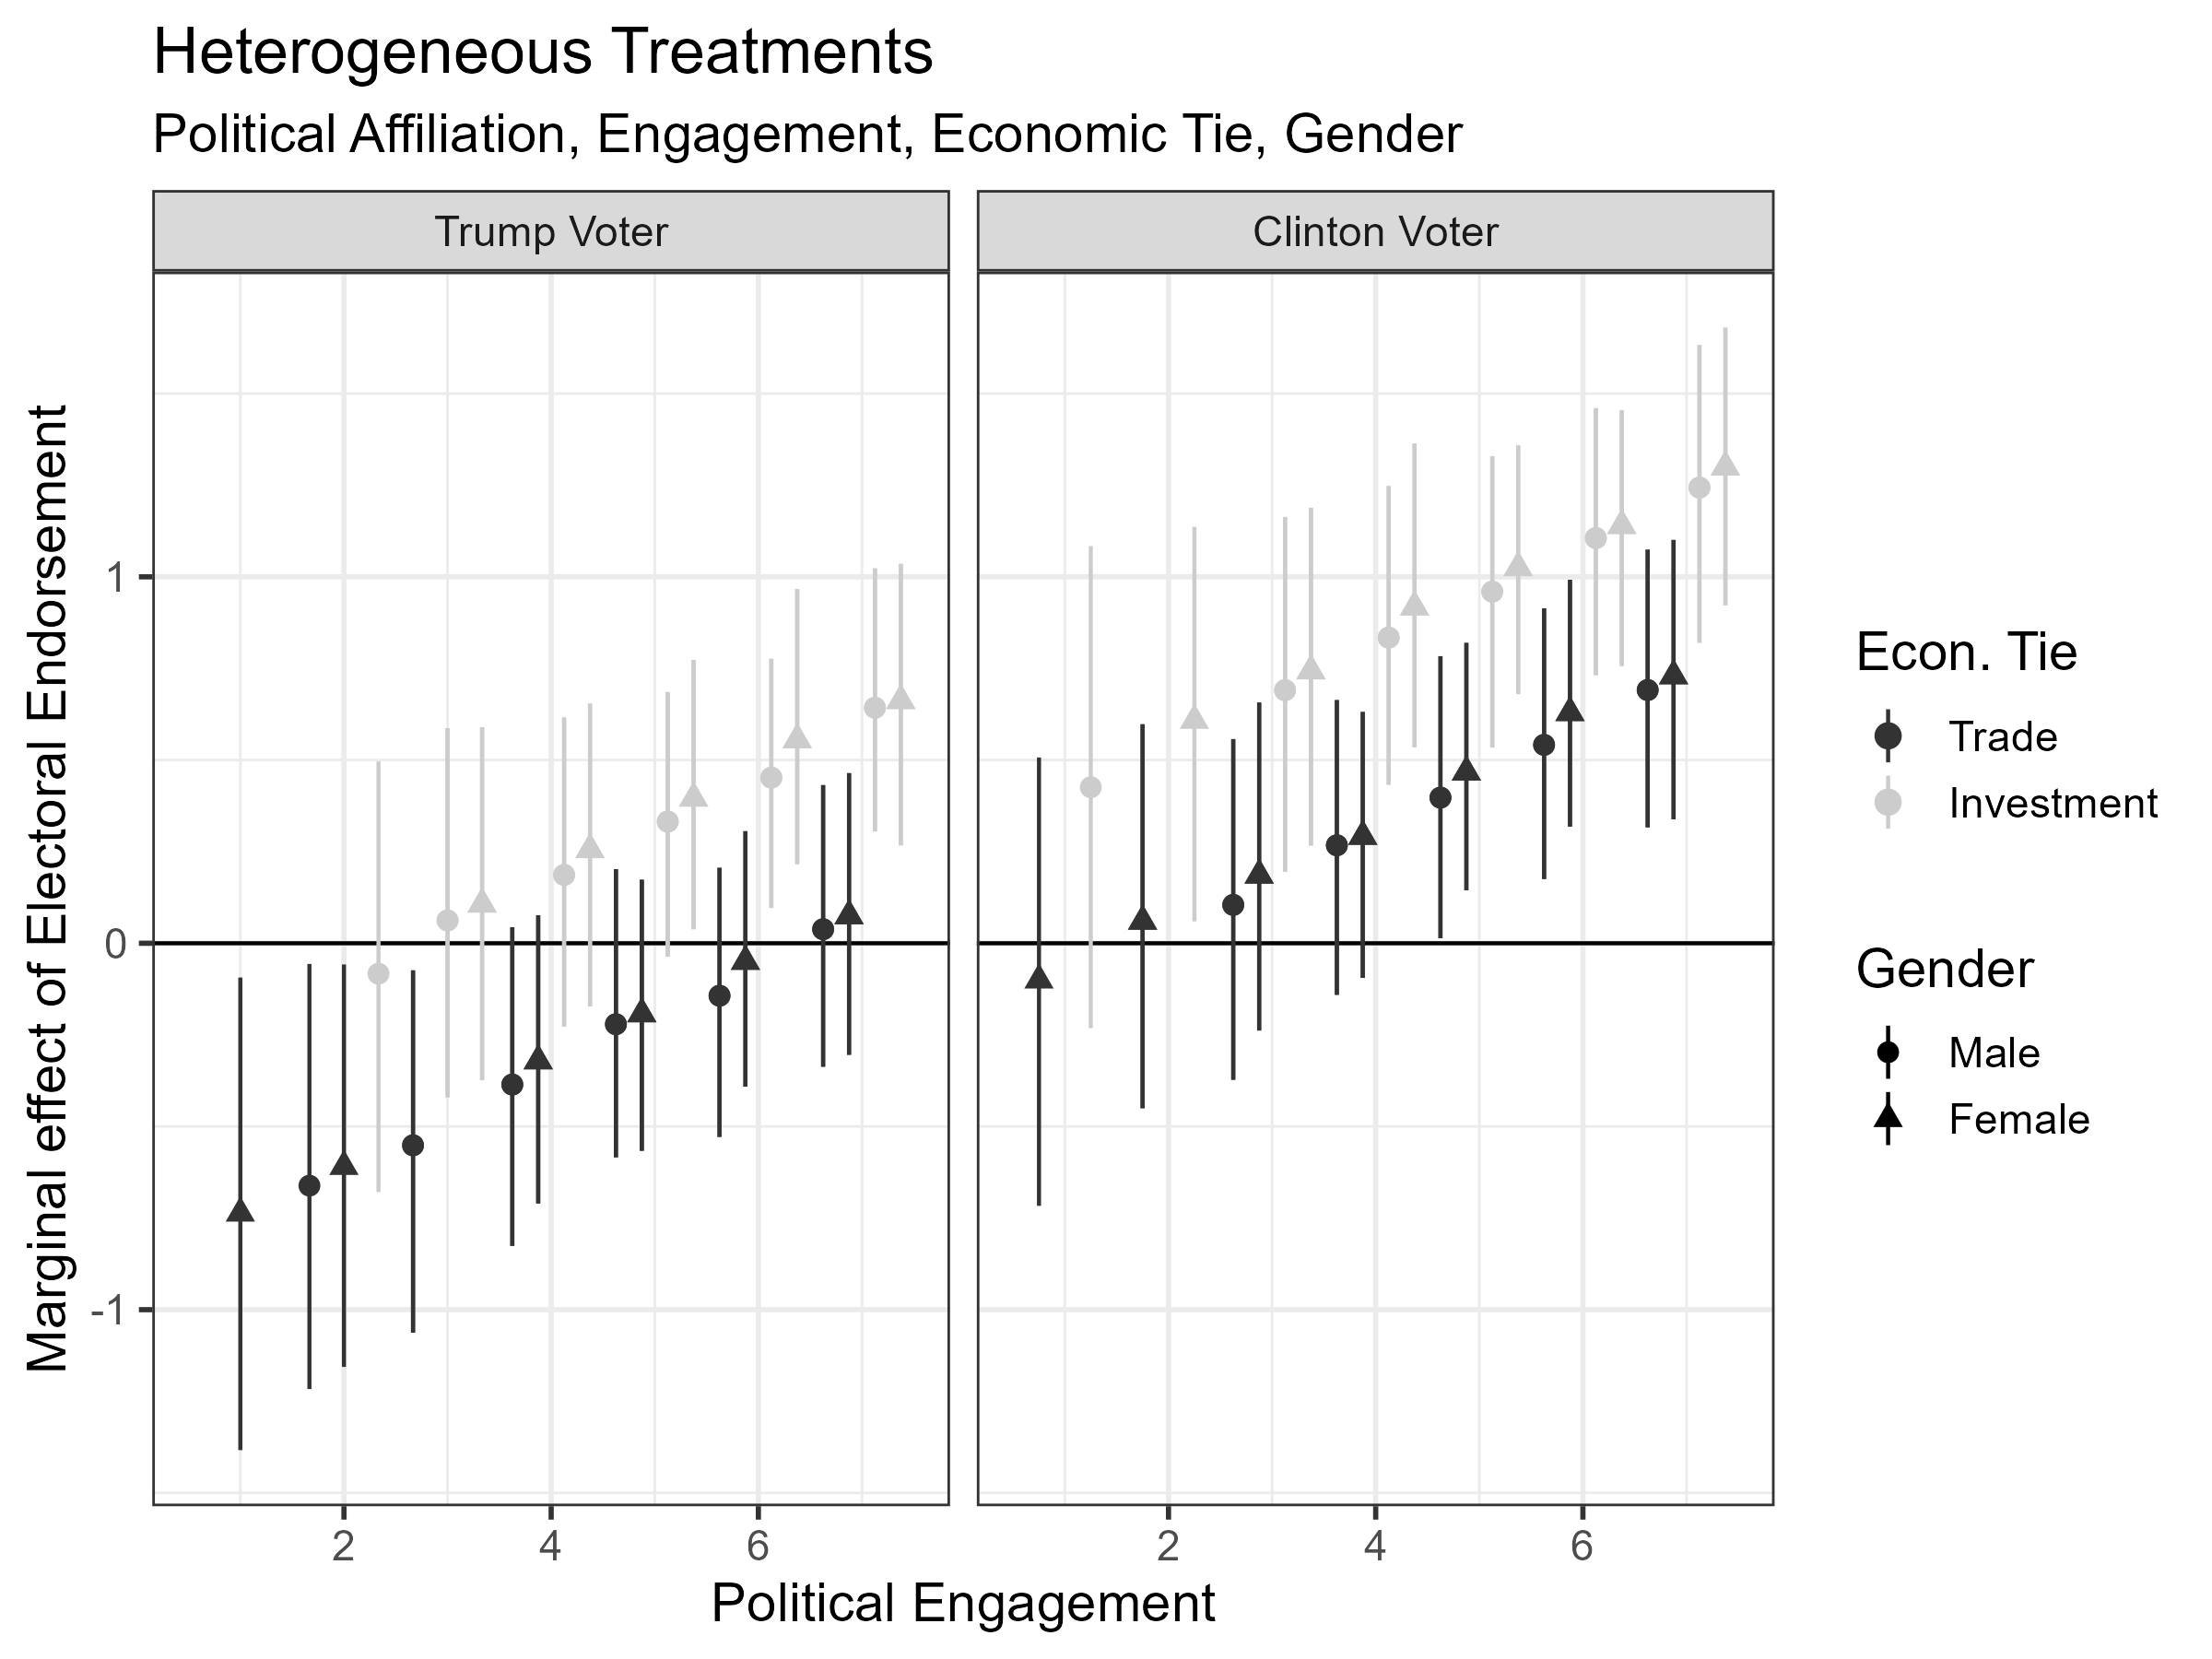
\includegraphics[width=0.95\textwidth]{bp-het-est.png}
	\caption{Heterogeneous effects of German side-taking in US elections on support for economic engagement with Germany. Each estimate reflects a treated group with a unique combination of other treatments and demographic characteristics.}
	\label{fig:bp-het-est}
\end{figure}


These estimates corroborate BP's findings, and also suggest that side-taking exerts the greatest influence on individuals who are highly engaged in politics. 
Clinton voters are more likely to support economic engagement with Germany when Germany has opposed Donald Trump. 
Conversely, some Trump voters oppose greater trade with Germany after the same side-taking. 
The impact of side-taking is also stronger for foreign investment than trade. 
Individuals are more willing to support investment than trade.


Side-taking exerts the most influence on individuals who are highly engaged in politics. 
Engaged Clinton voters respond most to German side-taking against Trump. 
Among these respondents, side-taking increases support for economic engagement by .5 or more, which is a large effect on an outcome that runs from one to four. 


\singlespace
 
\bibliography{../../MasterBibliography} 


\end{document}

\end{document}
